\documentclass[a4paper,10pt]{jsarticle}

% 数式
\usepackage{amsmath,amsfonts}
\usepackage{bm}
% 画像
\usepackage[dvipdfmx]{graphicx}
\usepackage{here}

\usepackage{listingsutf8,jlisting} %日本語のコメントアウトをする場合jlistingが必要
%ここからソースコードの表示に関する設定
\lstset{
  basicstyle={\ttfamily},
  identifierstyle={\small},
  commentstyle={\smallitshape},
  keywordstyle={\small\bfseries},
  ndkeywordstyle={\small},
  stringstyle={\small\ttfamily},
  frame={tb},
  breaklines=true,
  columns=[l]{fullflexible},
  numbers=left,
  xrightmargin=0zw,
  xleftmargin=3zw,
  numberstyle={\scriptsize},
  stepnumber=1,
  numbersep=1zw,
  lineskip=-0.5ex
}

\begin{document}

\title{コンパイラ演習課題3}
\author{坪井正太郎(101830245)}
\date{\today}
\maketitle
\section{}
\subsection{}
\[First_1(S)=\{a,b\}\]
\[First_1(A)=\{\epsilon,a\}\]
\begin{table}[htb]
  \centering
  \begin{tabular}{c|c|c|c|c|c|c|c|c|c}
      & (1)   & (2)   & (3)   & (4a)  & (4b)    & (4a)    & (4b)    & (4a)    & (4b)    \\ \hline
  S   &       &       & 0     & 0     & \{a,b\} & \{a,b\} & \{a,b\} & \{a,b\} & \{a,b\} \\
  A   &       &       & 0     & 0     & \{$\epsilon$,a\} & \{$\epsilon$,a\} & \{$\epsilon$,a\} & \{$\epsilon$,a\} & \{$\epsilon$,a\} \\
  a   &       & \{a\} & \{a\} & \{a\} & \{a\}   & \{a\}   & \{a\}   & \{a\}   & \{a\}   \\
  b   &       & \{b\} & \{b\} & \{b\} & \{b\}   & \{b\}   & \{b\}   & \{b\}   & \{b\}   \\
  e   & \{$\epsilon$\} & \{$\epsilon$\} & \{$\epsilon$\} & \{$\epsilon$\} & \{$\epsilon$\}   & \{$\epsilon$\}   & \{$\epsilon$\}   & \{$\epsilon$\}   & \{$\epsilon$\}   \\
  aSa &       & \{a\} & \{a\} & \{a\} & \{a\}   & \{a\}   & \{a\}   & \{a\}   & \{a\}   \\
  bAb &       & \{b\} & \{b\} & \{b\} & \{b\}   & \{b\}   & \{b\}   & \{b\}   & \{b\}   \\
  Sa  &       &       & 0     & 0     & 0       & \{a,b\} & \{a,b\} & \{a,b\} & \{a,b\} \\
  Ab  &       &       & 0     & 0     & 0       & \{a,b\} & \{a,b\} & \{a,b\} & \{a,b\} \\
  aS  &       & \{a\} & \{a\} & \{a\} & \{a\}   & \{a\}   & \{a\}   & \{a\}   & \{a\}  
  \end{tabular}
\end{table}

\newpage
\subsection{}
\[Follow_1(S)=\{\#,a,b\}\]
\[Follow_1(A)=\{b\}\]
\begin{table}[htb]
  \centering
  \begin{tabular}{c|c|c|c}
    & (1)    & (2)    & (3)        \\ \hline
  S & \{\#\} & \{\#\} & \{\#,a,b\} \\
  A & 0      & 0      & \{b\}     
  \end{tabular}
\end{table}

\section{}
\subsection{}
\[I_0=[[S'\rightarrow\circ S\#],[S\rightarrow\circ SA],[S\rightarrow\circ A],[A\rightarrow\circ a]] \]
\[I_1=[[S'\rightarrow S\circ\#],[S\rightarrow S\circ A],[S\rightarrow\circ A]]\]
\[I_2=[[S\rightarrow A\circ] ]\]
\[I_3=[[A\rightarrow a\circ]] \]
\[I_4=[[S\rightarrow SA\circ] ]\]

\subsection{}
\begin{figure}[H]
  \centering
  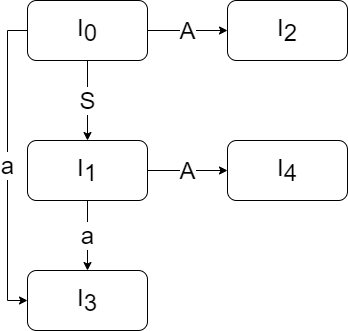
\includegraphics[width=10cm]{./01.png}
\end{figure}

\subsection{}
\[Follow_1(S)=\{\#,a\}\]
\[Follow_1(A)=\{\#,a\}\]

\subsection{}
\begin{table}[htb]
  \centering
  \begin{tabular}{c|c|c|c|c}
    & a  & \#     & S & A \\ \hline
  0 & s3 & \{\#\} & 1 & 2 \\
  1 & s3 & Acc    &   & 4 \\
  2 & r2 & r2     &   &   \\
  3 & r3 & r3     &   &   \\
  4 & r1 & r1     &   &  
  \end{tabular}
\end{table}

\end{document}
